\documentclass{article}
\usepackage[utf8]{inputenc}
\usepackage{amsmath}
\usepackage{amsfonts}
\usepackage{mathrsfs}
\usepackage{graphicx}
\usepackage{subcaption}
\usepackage[top=30truemm,bottom=30truemm,left=30truemm,right=30truemm]{geometry}


\title{Chaotic Dynamics: Homework 6}
\author{Kansuke Ikehara (Kansuke.Ikehara@colorado.edu)}

\begin{document}
\maketitle

\subsection*{Problem 1}
\subsubsection*{(a)}
Fig.\ref{q1a} shows a Poincare section with a hyper plane $\Sigma:t = nT_{0}$ where $T_{0}$ is the natural period of the system. The figure is supposed to plot only one point at the initial condition, since the hyper place is defined as a sequence of times whose interval is the natural period of the system. However, due to some numerical error, the resulting figure shows a trajectory of points emanating from nearby the initial place. 
\begin{figure}[h]
  \centering
  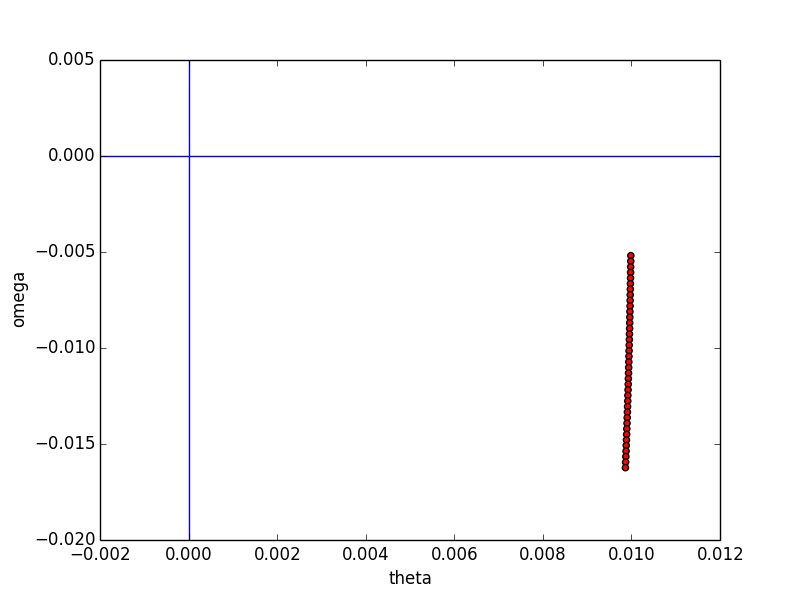
\includegraphics[height=2in]{figs/q1/q1a.png}
  \caption{Poincare section with hyper plane $\Sigma:t = nT_{0}$.}
  \label{q1a}
\end{figure}

\subsubsection*{(b)}
Fig.\ref{q1b} shows a Poincare section with a hyper plane $\Sigma:t = nT$ where $T$ is $\frac{T_{0}}{\pi}$. The difference between fig.\ref{q1a} and \ref{q1b} is the latter captures the entire trajectory of the pendulum's state, whereas the former only captures the trajectory around the initial condition. 

\begin{figure}[h]
  \centering
  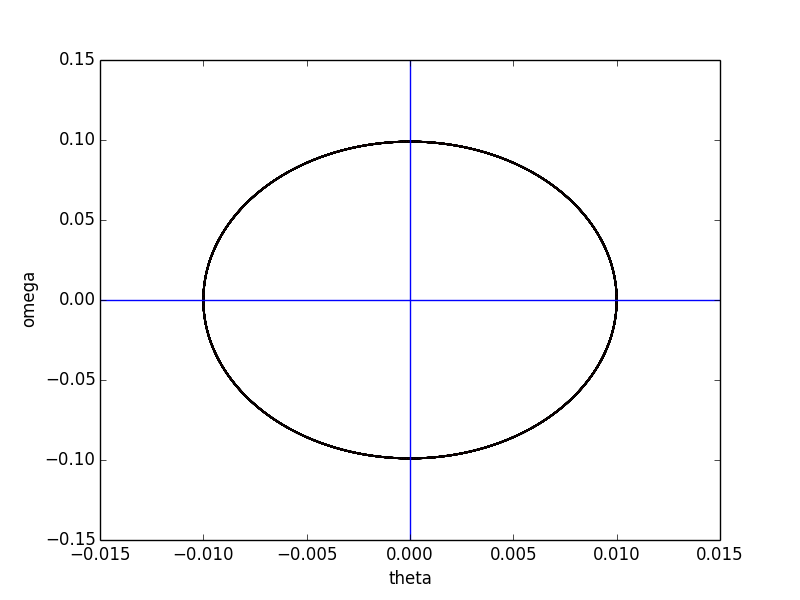
\includegraphics[height=2in]{figs/q1/q1b.png}
  \caption{Poincare section with hyper plane $\Sigma:t = nT$.}
  \label{q1b}
\end{figure}

\subsubsection*{(c)}
Fig.\ref{q1c} shows the Poincare section $\Sigma:t = nT_{drive}$ where $T_{drive}$ is the period of the driving force. 

\begin{figure}[h]
  \centering
  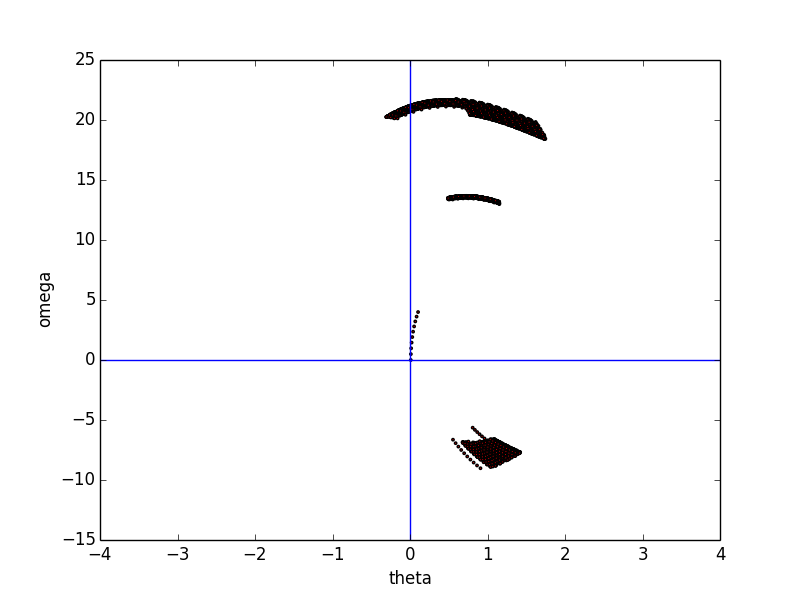
\includegraphics[height=2in]{figs/q1/q1c_delta_t_0005.png}
  \caption{Poincare section of a chaotic attractor of the driven pendulum.}
  \label{q1c}
\end{figure}

\subsubsection*{(d)}
As we increase the step size of the ODE solver while keeping the time span covered the same, we gradually observe the entire picture of Poincare section of the chaotic attractor. This is due to the fact that the larger step size of ODE enables it to cover the the state-space fully, so when we have a Poincare section, we can see the entire picture of the underlying structure. 

\subsection*{Problem 2}
\subsubsection*{(a)}
For part (c), the resulting Poincare section of the linear-interpolation method is almost identical to what we observe in the question1's (c). See fig.\ref{q2c}. For part (d), however, the resulting Poincare section is a little bit different from the one with non-interpolation. See Figs. \ref{q21} and \ref{q22}.

\begin{figure}[h]
  \centering
  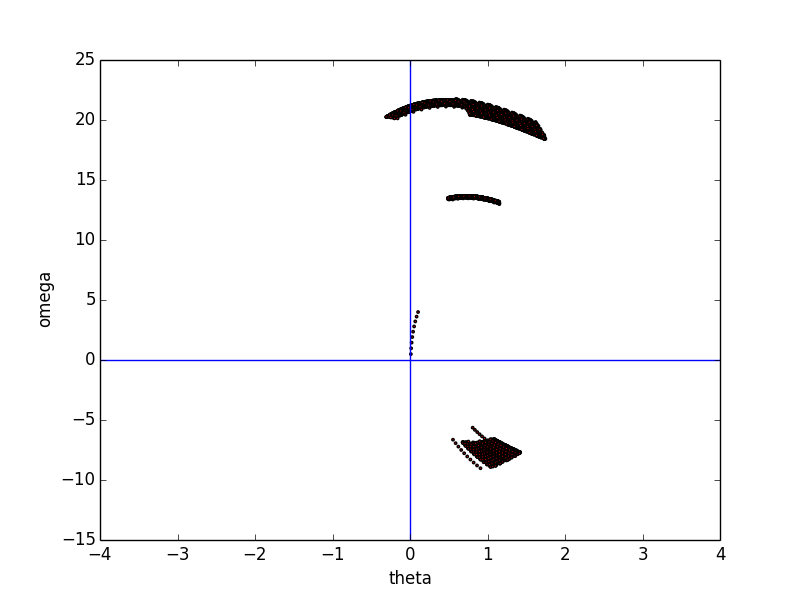
\includegraphics[height=2in]{figs/q2/c.png}
  \caption{Poincare section of a chaotic attractor of the driven pendulum derived by a linear-interpolated method.}
  \label{q2c}
\end{figure}

\begin{figure}[h]
\centering
\begin{subfigure}{.5\textwidth}
  \centering
  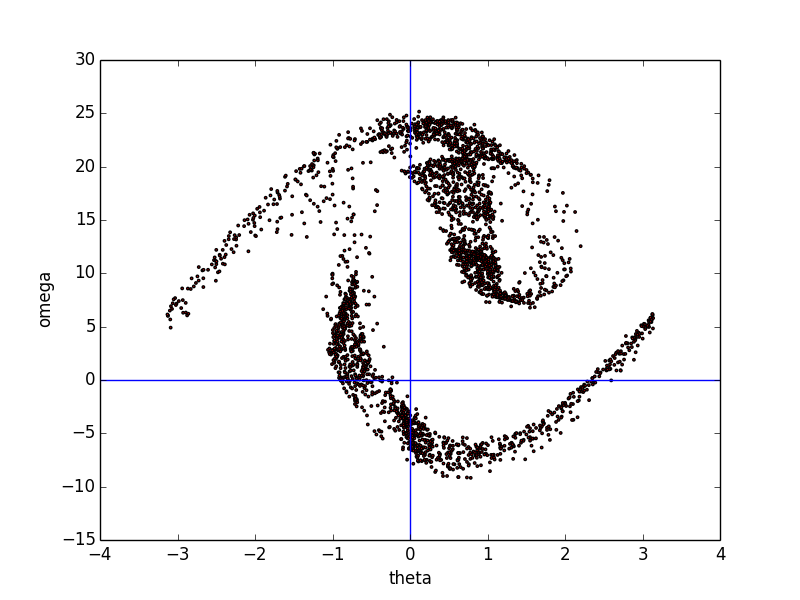
\includegraphics[height=2in]{figs/q2/non_interpolation.png}
  \caption{Non interpolated}
  \label{q21}
\end{subfigure}%
\begin{subfigure}{.5\textwidth}
  \centering
  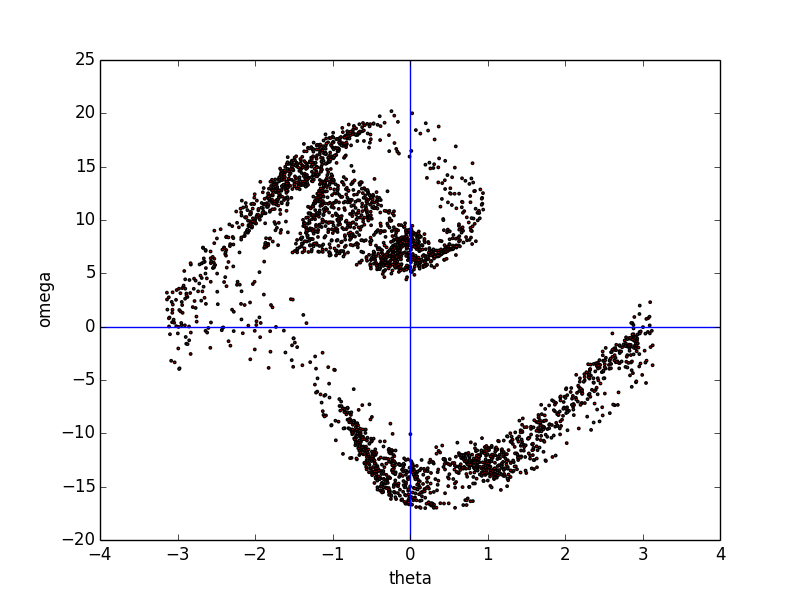
\includegraphics[height=2in]{figs/q2/interpolation.png}
  \caption{Interpolated}
  \label{q22}
\end{subfigure}
\caption{Poincare sections of: 1.non-interpolated and 2.interpolated.}
\label{q2}
\end{figure}

\subsection*{Problem 3}
Figs.\ref{q31} and \ref{q32} show the Poincare sections for the Lorenz attractor with $y = 20$ and $y =2x$, respectively.

\begin{figure}[h]
\centering
\begin{subfigure}{.5\textwidth}
  \centering
  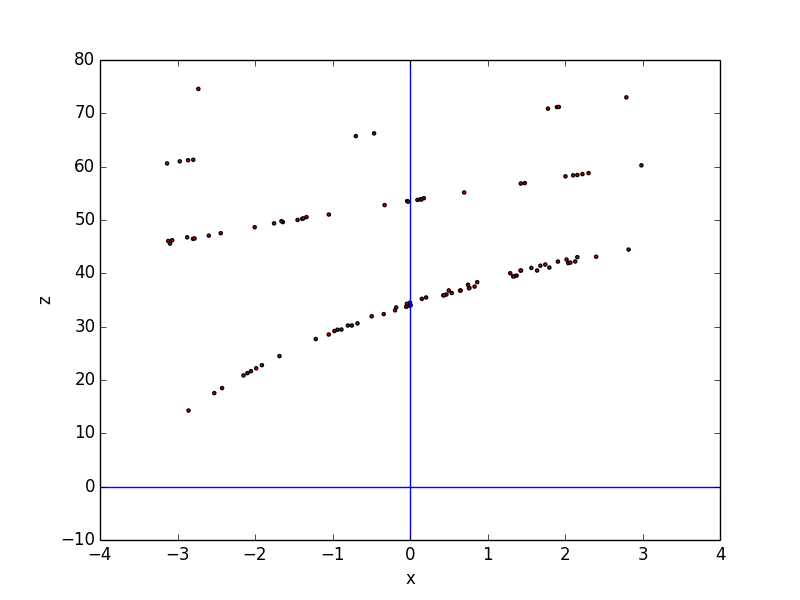
\includegraphics[height=2in]{figs/q3/q3a.png}
  \caption{$y = 20$}
  \label{q31}
\end{subfigure}%
\begin{subfigure}{.5\textwidth}
  \centering
  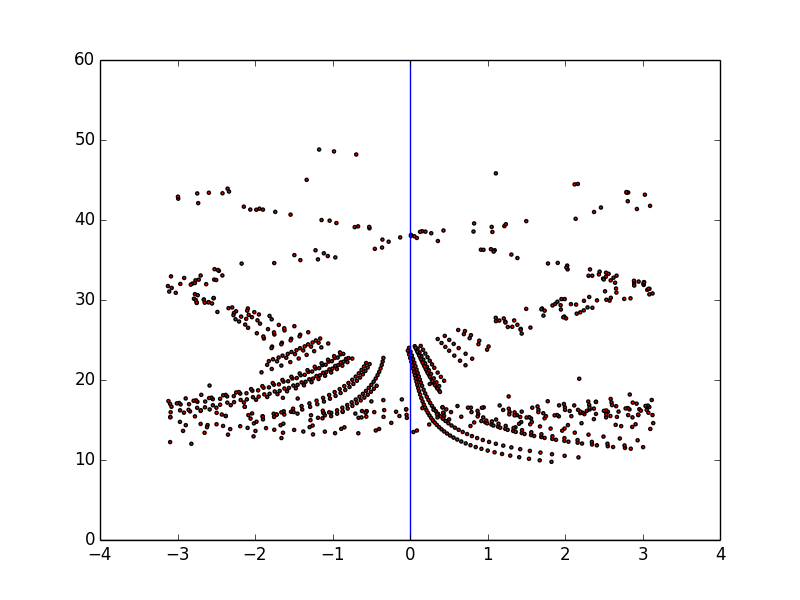
\includegraphics[height=2in]{figs/q3/q3b_correct.png}
  \caption{$y = 2x$}
  \label{q32}
\end{subfigure}
\caption{Poincare sections for each setting.}
\label{q3}
\end{figure}

\end{document}












